\subsection{System configuration}
We apply the robust MS stability condition to the robustness analysis of the following inverted pendulum robot example. We assume that the sensor can ideally measure some of the system's outputs without additive noises. However, we are interested in analyzing the effects of intermittent attention. This can model a user paying discontinuous attention to the device or that the sensor is connected to the controller over an unreliable network. We want to study how the robustness to unmodeled dynamics is affected by unreliable networks and vice versa.  

\begin{figure}[h]
    \centering
    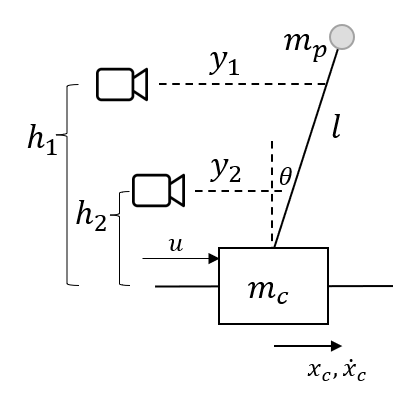
\includegraphics[width = 0.5\linewidth]{figures/RMSSfigure/IPmodel.png}
    \caption[1-D inverted pendulum model]{$m_c$ is the mass of the cart. The pendulum is ideally modeled as a light pole with a concentrated mass $m_p$ at its tip. The driving force on the cart $u$ is the control input to the system.}
    \label{fig:pendulumplant}
\end{figure}

Equations of motion in continuous time are given as~\eqref{eqn:EoMPendulumCT}, adapted from \cite{leong2016understanding}.
\begin{subequations}\label{eqn:EoMPendulumCT}
\begin{align}
(m_c+m_p)\ddot{x}_c+ m_p l (\ddot{\theta}-\dot{\theta}^2 \sin{\theta}) & = u  \\
m_p (\ddot{x}_c\cos{\theta}+l\ddot{\theta}-g \sin{\theta})=0
\end{align}
\end{subequations}
We assume we have two sensors measuring the horizontal motion of two points on the pendulum. The measurements are given by,
\[
y_1 = h_1 \tan \theta + x_c;\quad y_2 = h_2 \tan \theta + x_c;\quad h_1 > h_2.
\]
We highlight that the system is observable from either of these channels. The controller is causal and provides the driving force $u$ to the cart to maintain the pendulum's stability based on the measured signals.  





% {\color{red} gain and phase margins (are not imprecise) are a measure of the uncertainty of the system! More importantly, we are using disk uncertainty, which is a generalization of classical gain and phase margins}
Let the state be $x=[\theta,\dot{\theta},s, \dot{s}]^T$. Linearizing the dynamic model about \(x^T=
\left[
\begin{array}{cccc}
    0 & 0 & 0 & 0\\
\end{array}\right]\)
gives the continuous time differential equation:

\begin{subequations}\label{eqn:EoMPendulumCT_ss}
\begin{align}
P_{\rm{CT}}\colon \dot{x}
= & \left[
\begin{array}{cccc}
    0 & 1 & 0 & 0 \\
    \frac{(m_c + m_p) g}{m_c l} & 0 & 0 & 0 \\
    0 & 0 & 0 & 1 \\
    -\frac{m_p g}{m_c}  & 0 & 0 & 0 
\end{array}\right]
x +
\left[
\begin{array}{c}
    0 \\ -\frac{1}{m_c l} \\ 0 \\ \frac{1}{m_c}\\
\end{array}\right] u \\
y = & \left[
\begin{array}{c}
    y_1 \\ y_2 
\end{array}\right]
= \left[
\begin{array}{cccc}
    h_1 & 0 & 1 & 0 \\
    h_2 & 0 & 1 & 0
\end{array}\right]
x
\end{align}
\end{subequations}

% \begin{subequations}\label{eqn:EoMPendulumCT_ss}
% \begin{align}
% P_{\rm{CT}}\colon \left[
% \begin{array}{c}
%     \ddot{\theta} \\ \dot{\theta} \\ \dot{x}_c \\ \ddot{x}_c\\
% \end{array}\right]
% = & \left[
% \begin{array}{cccc}
%     0 & 1 & 0 & 0 \\
%     \frac{(m_c + m_p) g}{m_c l} & 0 & 0 & 0 \\
%     0 & 0 & 0 & 1 \\
%     -\frac{m_p g}{m_c}  & 0 & 0 & 0 
% \end{array}\right]
% \left[
% \begin{array}{c}
%     \theta \\ \dot{\theta} \\ x_c \\ \dot{x}_c\\
% \end{array}\right]+
% \left[
% \begin{array}{c}
%     0 \\ -\frac{1}{m_c l} \\ 0 \\ \frac{1}{m_c}\\
% \end{array}\right] u \\
% \left[
% \begin{array}{c}
%     y_1 \\ y_2 
% \end{array}\right]
% = & \left[
% \begin{array}{cccc}
%     h_1 & 0 & 1 & 0 \\
%     h_2 & 0 & 1 & 0
% \end{array}\right]
% \left[
% \begin{array}{c}
%     \theta \\ \dot{\theta} \\ x_c \\ \dot{x}_c\\
% \end{array}\right]
% \end{align}
% \end{subequations}

We adopt zero-order hold discretization to obtain the discrete-time state-space representation.


Stochastic communication intermittency occurs in each communication channel between sensors and the controller, i.e. controllers receive intermittent \(y_1\) and \(y_2\) signals.
Deterministic model uncertainties may arise from multiple sources, such as gain fading, unmodeled dynamics, and model parameter errors. We aim to assess the overall tolerance to these uncertainties. So we choose an entrance to the $\Delta$ block, which describes the disk margin of the open-loop interconnection between the plant and controller. It is shown in Appendix~\ref{appsec:RMSS}.

% $$
% x^+=A x + B u;\ y=Cx
% $$
% {\color{red} then next section is a bit problematic. 1) we have not been focused on design, so why do we focus on it now? The controller should be given, and motivated, and if justified it need to be explain correctly.}  
\subsection{Controller Design}

% {\color{red} the above sentence is illogical, if there were a design method it would be automatically based on an analysis method. Moreover, why don't we use the D-K design method for mu?}$\surd$




Motivated by~\cite{Jeff2005Packet}, we consider a controller architecture consisting of a controller and a ``receiver'' that monitors the communication channel status and imputes missing signals, shown in Figure~\ref{fig:Ctrl_Receiver}.
\begin{figure}[htbp]
    \centering
    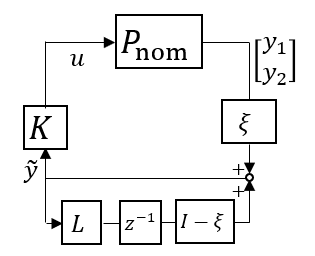
\includegraphics[width=0.5\linewidth]{figures/RMSSfigure/Ctrl_Receiver.png}
    \caption[]{The schematic of the controller that compensates for the intermittent measurements.}
    \label{fig:Ctrl_Receiver}
\end{figure}
$P_\mathrm{nom}$ is the nominal plant, $K$ is the output feedback controller. $L$ is the ``receiver'' which imputes the missing signals. $\xi=\mathrm{diag}(\xi_1,\xi_2)$, $\xi_1$ and $\xi_2$ are IID stochastic numbers which take value from $\{0,1\}$ at each time step. For example, $L = I_2$ is equivalent to a zero-order hold: the output measurement from the last time step replaces the signal if it has dropped.

Through a sequence of block diagram transformations, the design of $[K;L]$ is equivalent to the synthesis of a controller for the system in Figure~\ref{fig:CLRMSSsyn}, where $\hat{K} = K(I- z^{-1} L)^{-1}$, $\hat{L} = L(I- z^{-1} L)^{-1}$. \([\hat{K};\hat{L}]\) can be seen as a stabilizing controller for the augmented plant \(\left[P,-z^{-1} I_2\right]\).


We now reintroduce the model uncertainty and signal intermittency into this closed-loop system; see Figure~\ref{fig:CLRMSSsyn}(b). $\bar{\Delta}\colon y\mapsto v$ is a mean \(0\) stochastic multiplicative block whose variance is determined solely by the packet drop probability $e$. $\Delta\colon q\mapsto p $ is an \(\mathcal{H}_\infty\) norm-bounded LTI uncertainty block, and its maximal size captures the open-loop disk margin of interconnection of plant and controller.

\begin{figure}[htbp]
    \centering
    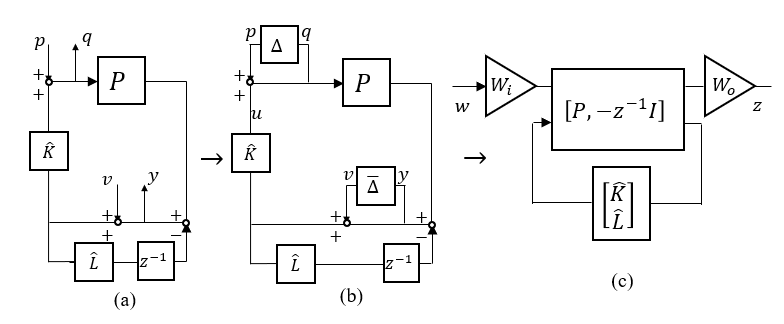
\includegraphics[width =1\linewidth]{figures/RMSSfigure/completeCLsys.PNG}
    \caption[mean system, robust analysis system model and generalized plant.]{(a) is the mean system. (b) is the complete system with stochastic and deterministic uncertainties. $\bar{\Delta} =\mathrm{diag}(\delta_{s_1},\delta_{s_2})$, $\E {\delta_{s_i}} = 0$ are IID, variance $\mathrm{var}(\delta_{s_i}^2) = e/(1-e)$, with $e$ probability to take $-1$ and $1-e$ probability to take $e/(1-e)$. On the other side, $\|\Delta\|_\infty<\eta$. (c) is the generalized plant used for \(\mathcal{H}_\infty\) synthesis. $w$ are the noises, while $z$ are the performance outputs. $W_i$ is the weight matrix for inputs. $W_o$ is the weight matrix for outputs.}
    \label{fig:CLRMSSsyn}
\end{figure}

Within the robust mean square analysis framework, we aim to find \([\hat{K};\hat{L}]\) to minimize
\[
\max_{\Delta \in \eta \mathcal{B}_{\bm{\Delta}}^{\mathrm{LTI}}} \ \rho\big(\tilde{T}_{yv}(\Delta)\big),
\]
which represents the worst-case spectral radius of the $\mathcal{H}_2$ matrix associated with the transfer function from $v$ to $y$.
However, such optimal controller design remains an open problem. Herein, we evaluate the limitations of an existing controller.  

As an reasonable approximation, we instead adopt \(\mathcal{H}_\infty\) synthesis to minimizes the weighted norm:
\[
\|W_o T W_i\|_\infty,\quad T \colon 
\begin{bmatrix}
p \\ v
\end{bmatrix} \mapsto 
\begin{bmatrix}
q \\ y
\end{bmatrix}
\]
Need more details on how the $\mathcal{H}_\infty$ controller is designed, see Appendix~\ref{appsec:RMSS}. 

By finely tuning the weight matrix $W_i$ and $W_o$, we can obtain a satisfactory controller.
In Figure~\ref{fig:CLRMSSsyn}.b, the mean system has an equivalent loop transfer function of $\hat{K}(I+z^{-1}\hat{L})^{-1}P$. From the controller we've designed, the loop transfer function has properties shown in Table~\ref{tab:margin}. The margins are sufficient. 
% We can conclude that this controller is robust against model uncertainty. 
\begin{table}[h]
    \caption{Properties of the open loop system}\label{tab:margin}
    \centering
    \begin{tabular}{cc|cc}
    \hline
        Property  & Value & Property  & Value\\
    \hline
        Gain margin & $[0.5247,1.9055]$ & Disk margin & $ 0.6233$\\
        Phase margin & $[-34.62,34.62]\deg$ & $\mathcal{H}_\infty$ norm & 1.4627 \\
        \hline
    \end{tabular}
\end{table}


We implement the discrete-time controller on the nonlinear continuous-time plant using MATLAB Simulink. Before applying our framework to find the robustness margin, we validate the controlled inverted pendulum under two scenarios. 
In the first scenario, there are no perturbations: all sensor measurements reach the controller, and the dynamic model is accurate. 
In the second scenario, each measurement on both channels has a $0.4$ probability of dropout, and the model is subject to a perturbation $\Delta$ aligned with the worst-case direction, with $\|\Delta\| = 0.2393$. 
The initial conditions are both set as \([0.05,0.02,0,0.1]^\top\).
The simulation results are shown in Figure~\ref{fig:impulse_resp}.

We can see that the system stabilizes in both configurations, this shows that the controller tolerates the packet drop and model uncertainty decently.

\begin{figure}[ht]
    \centering
    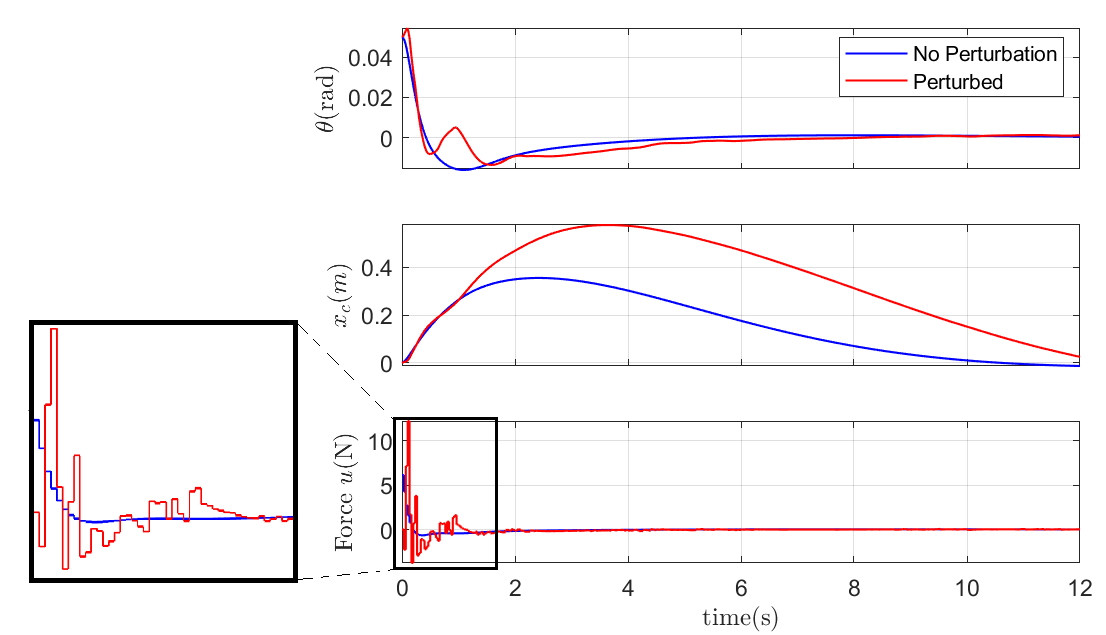
\includegraphics[width = 0.95\linewidth]{figures/RMSSfigure/states_plot_detailed.png}
    \caption[Cart-pole impulse response]{The impulse response of a initial cart velocity $\dot{s}=0.1$ without model perturbation and packet drops. The system recovers zero state in about 10s.}
    \label{fig:impulse_resp}
\end{figure}

\subsection{Robust Mean Square stability analysis}




 % Its disk margin is $0.6335$. Its phase margin is $[-35.15\deg,35.15\deg]$.


Write the system in the expression of equation (\ref{Discrete_statespace_Mix}). Compute the $M(e^{j\omega})$ by \eqref{eqn:constrM} and \eqref{constrM_i} and apply Theorem~\ref{thm:RMSSsuff}. To implement it in numerical tools, we can only have finite constraints. Therefore, we uniformly sample $N=100$ points from $[0,2\pi)$ and approximate the integral LMIs by a finite sum. We get $2N$ different constraints and 2 sum constraints instead of the integral constraint in Theorem \ref{thm:RMSSsuff}.
\begin{subequations}
\begin{align}
M_i(e^{j\omega(k)})
\left[
\begin{array}{cc}
    \tilde{X}_i(\omega(k)) & 0 \\
    0 &\beta
\end{array}\right]
[M_i(e^{j\omega(k)})]^\hermconj & < \left[
\begin{array}{cc}
    \tilde{X}_i(\omega(k)) & 0 \\
    0 & w_i(\omega(k))
\end{array}\right],\\ 
\frac{1}{N} \sum_{k=1}^{N}w_i(\omega(k)) \leq \gamma \beta_i, &  \quad i=1,2; \\
\omega(k) =\frac{2k\pi}{N}+\alpha,& \quad k\in \mathcal{H}_N.
\end{align}
\end{subequations}


By checking the feasibility of these LMIs, we can find the maximum $\gamma$ corresponding to different deterministic size $\eta$, i.e. the inverse of maximum allowed variance in $\delta_{s_i}$. Since $\frac{1}{\gamma} = \sigma_{\max}^2 =\frac{e}{1-e}$,
$$
e=\frac{1}{\gamma+1}.
$$
Figure~\ref{fig:eta_e} plots the largest allowed probability of packet drop against the model uncertainty's \(\mathcal{H}_\infty\) upper bound $\eta$. We apply the same controller and consider three scenarios: (i) the first output channel is perfect (i.e., without intermittency), (ii) the second output channel is perfect, and (iii) both channels experience intermittent dropouts.
\begin{figure}[h]
    \centering
    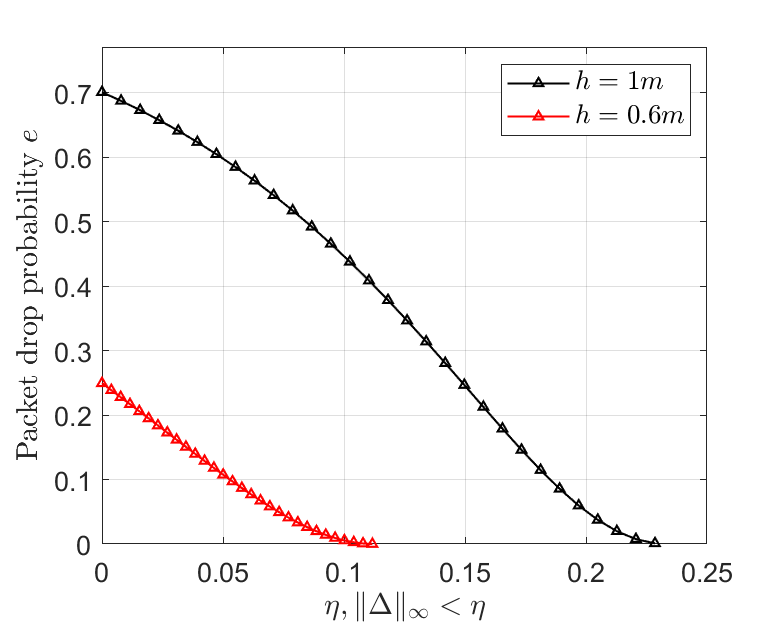
\includegraphics[scale=0.8]{figures/RMSSfigure/eta_e_plot.png}
    \caption[Robustness against both stochastic process and model uncertainty]{The relationship between the maximum drop-out probability against radius of disk uncertainty.}
    \label{fig:eta_e}
\end{figure}

Basically, the nominal system with \(0\) drop-out probability achieves the largest disc robustness. As the system is subject to increasing drop-out, its robustness to deterministic disc uncertainty diminishes. This figure numerically demonstrates the interplay between the two different type of uncertainty. Finally, for a maximum dropout probability of $44\%$, the system is fragile to deterministic input uncertainty. 